\section{Experiments}
\label{sec:experiments}

\TODO { Comparing with other's aspect extraction results, 
for example using the human annotated feature words. }

\TODO { Measure the semantic similarity between our extracted top aspect words 
and the groundtruth aspects. 
For example, find K nearest neighbors of our extracted aspect words, 
when K=3, K=5, K=10, how many percent of the groundtruth aspects are matched?
}

\TODO { End to end aspects summarization, other's results ? }

In this section, we present the results of three experiments. 
The first one is a comparison of methods for obtaining sentence vectrs. 
In the first step of our framework, i.e., sentence clustering, 
sentence representation is crucial to the performance 
and hence critical to overall performance of the framework. 
In particular, we need a vector representation 
that accurately captures the semantic similarity between sentences, 
so we test the performance of the methods on a sentence similarity 
prediction task. 
The second experiment is the comparison of our framework
with a number of baselines including the state-of-the-art approaches
in the end-to-end aspect extraction task.
The third experiment is a complete aspect-based summarization using our model.

\subsection{Experiment 1: Aspects Extraction Results}


We can see that, although with fewer parameters, 
paragraph vectors outperforms LSTM on this task. 
This is probably because the last hidden vector of LSTM is not 
a proper representation of the sentence for the semantic similarity task, 
due to its emphasis on the last seen words as opposed to earlier words. 
The performance of different sentence vectors is included in the next experiment.


\subsection{Experiment 2: End-to-end Evaluation of Aspect Extraction}

In this experiment, we evaluate the framework on the real-world application:
aspect extraction from user reviews. 

\subsubsection{Data}

The data we use in this experiment was gathered from various e-commerce 
websites, including amazon.com, tripadvisor.com, etc. 
The reviews are about 15 categories of product or service. 
The review content is plain English text and we do not use any labels 
for training our model. We use human labels for evaluation. 
The product categories, their sources and the sizes of the review datasets
are summarized in \tabref{table:dataset}

\begin{table}[th]
\small
\centering
\caption{Dataset summary.} 
\label{table:dataset}
\begin{tabular}{|c|c|c|c|}
\hline
Product type & Source & No. of Reviews & No. of Words \\ \hline \hline
hotel        & TripAdvisor & 27145   & 210 \\\hline
mobile phone & Amazon & 3716    & 136 \\\hline
mp3 player   & Amazon & 2745    & 128 \\\hline
laptop       & Amazon & 5471    & 97  \\\hline
transportation & Yelp & 3077  & 131 \\\hline
restaurant   & Yelp & 4016    & 176 \\\hline
\end{tabular}
\end{table}


For evaluation, we ask 5 college students proficient with English 
to annotate ground truth
aspect words for each product category. For each category, 
we ask them to provide 5 different words that cover the most important 
aspects of the corresponding product or service. The labels provided by the
5 annotators are aggregated together without removing duplicated words, 
so we have 25 words in total. 
When evaluating the models, 
we compare the 5 aspect words generated by the models with those provided 
by the annotators. 
We calculate the portion of words among the 25 labels that 
are correctly generated by the model as the accuracy of the model.
The ground-truth labels for two product categories are shown 
in \tabref{table:labels}.


\begin{table}[th]
\centering
\caption{Labels for hotel and shopping. Each row is provided by one annotator.}
\label{table:labels}
\begin{tabular}{|c|l|}
\hline
\multirow{5}{*}{hotel}
& room price location service utility \\
& room service price food location  \\
& sleep service room price location  \\
& location price bedroom bath staff  \\
& room price bath staff location  \\\hline

\multirow{5}{*}{shopping}
& location product service price environment \\
& product price service location ambience \\
& price food location size facility \\
& sales location food service environment \\
& price location service facility food \\\hline
\end{tabular}
\end{table}

\subsubsection{Parameter Tuning}

In this section we conduct experiments to determine the best set of
parameters of our model, most importantly the constants $N$, $M$, $C$.

\textbf{Number of Sentence Clusters ($N$)}

In the first clustering step we use a k-means to cluster the sentences,
where each cluster should contain sentences about similar aspects.
We need to determine the number of clusters, $N$.
We use an empirical elbow method to determine $N$, 
we plot the total distance between each point and its corresponding center,
a.k.a. the loss, with different choices of $N$, 
as shown in \figref{fig:differentn}.
Note that we are not concerned with the number of expected aspects 
in this experiments. 
As we can see from \figref{fig:differentn},
to give the smallest loss, the number of sentence clusters should be
10 or 11.  Therefore, in the following experiments, we choose $N$ to be 10.

\begin{figure}[t!]
\centering
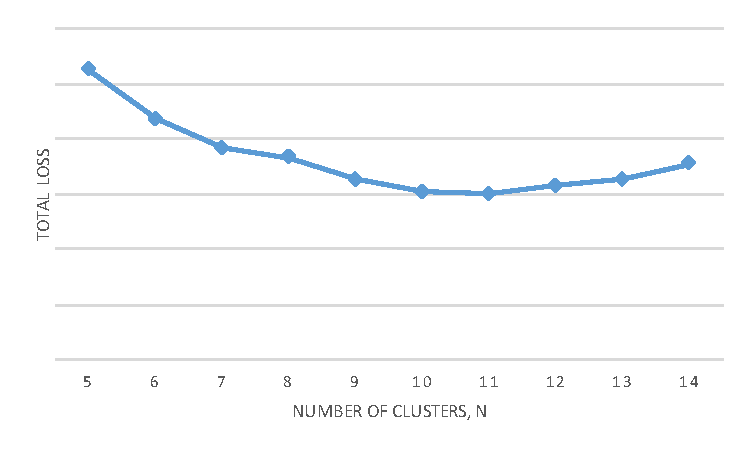
\includegraphics[width=0.9\columnwidth]{figures/differentn}
\caption{Selecting the number of cluster for k-means.}
\label{fig:differentn}
\end{figure}

\textbf{Number of LDA Topics ($M$)}

LDA in our model serves the purpose of isolating the 
noisy topics and resolving the overlaps between aspects.
In our experiments we find that different number of LDA topics
doesn't have much effect on the end-to-end performance.
As an example, the aspect extraction accuracy with different $M$
on hotel reviews are shown in \tabref{table:differentm}.
Consider the 25 words that we compare our model agains,
the difference between the three numbers is only 
1 out of 25 words.
In our experiments, $M$ is fixed to 10.

\begin{table}[th]
\centering
\caption{The effect of different number of LDA topics}
\label{table:differentm}
\begin{tabular}{|c|c|c|c|}
\hline
$M$ & 5 & 8 & 10 \\\hline
Accuracy & 19/25 & 18/25 & 19/25 \\\hline
\end{tabular}
\end{table}

\textbf{Redundant Clusters ($C$)}

As mentioned in \secref{sec:topic_clustering}, 
we generate $C$ aspect clusters before ranking the clusters and the words, where $C$ is larger than $K$.
In this section we demonstrate the effect of these redundant clusters.
In \figref{fig:differentc}, we show the accuracy with different 
redundancy $C-K$, 
ranging from 0 to 4, with numbers of expected aspects ranging from 3 to 7.
It can be seen that 2 redundant clusters is sufficient and 
more redundancy can't improve the performance.

\begin{figure}[th]
\centering
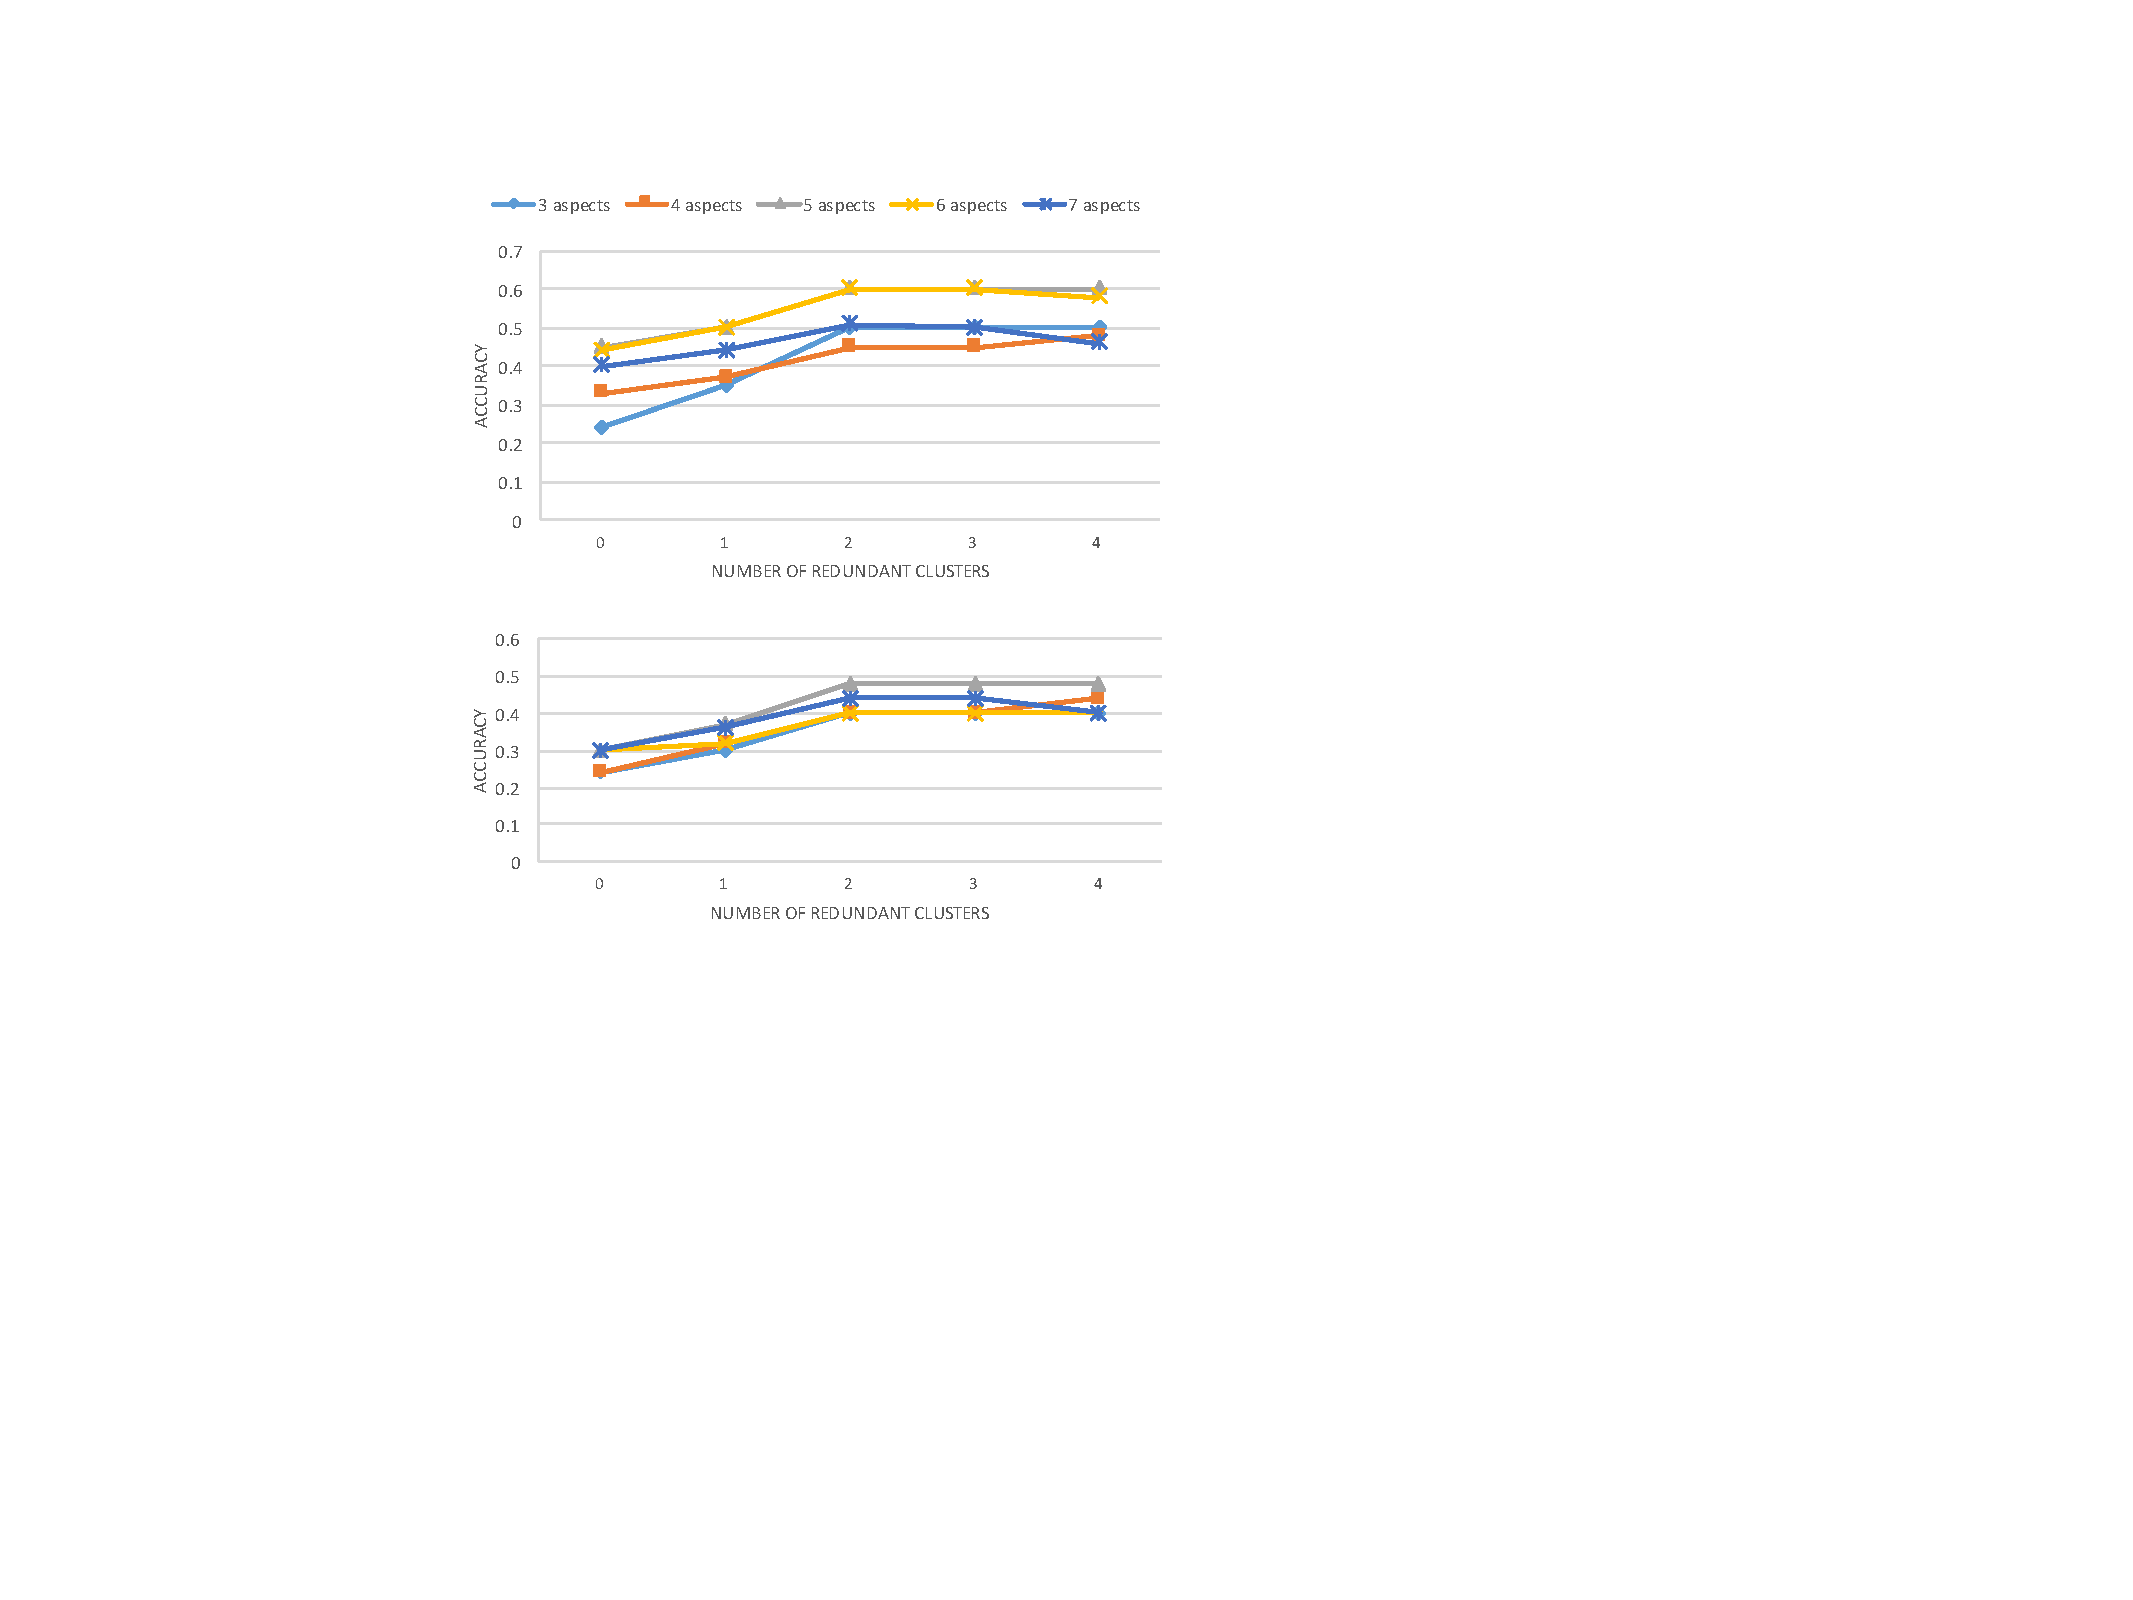
\includegraphics[width=0.9\columnwidth]{figures/differentc}
\caption{The performance of different models when varying the 
number of redundant aspects. Top: hotel reviews. Bottom: gym reviews.}
\label{fig:differentc}
\end{figure}



\subsubsection{Models}

In this section we introduce the models used in our end-to-end comparison.
We compare 6 models in our experiments, 
LDA as a simple baseline, 
D-PLDA \cite{moghaddam2012design} as a representative for joint aspect-sentiment models, 
MG-LDA \cite{titov2008modeling} as a representative for aspect extraction topic model,
and two variations of our model Ours(LSTM) and Ours(PV). 
We run the 4 models on the review data of each product type sepereately. 
For the main experiment, the number of aspects is fixed to 5.

\paragraph{LDA}
We use LDA as a simple topic model baseline for our model. 
We treat each review as a document and run on the whole corpus (single product type). 
The number of topics is set to 5 for model comparison.

\paragraph{D-PLDA}
D-PLDA \cite{moghaddam2012design} is an LDA variation designed specifically for modeling user reivews. 
In D-PLDA, only opinion phrases are modeled, 
and the nouns and the phrases are controlled by two seperate hidden parameters 
where there is a dependency from hidden parameter for adjectives to the one for nouns.
We use D-PLDA as a representative for models with join aspect and sentiment inference.


\paragraph{MG-LDA}
To compare our model with a popular, well-performning model designed for aspect extraction, 
we choose MG-LDA \cite{titov2008modeling}. 
MG-LDA also models topics at different grandularities. 
For model comparison, the number of local topics (aspect topics) is set to 5, 
the number of global topics is set to 30 (ignored in evaluation).

\paragraph{Our models}
For sentence vectors (both LSTM and PV), the dimensionality is set to 300. The number of sentence-level clusters is set to 10; the number of LDA topics is 10; the number of final word clusters in the clustering phase is 7 and is later reduced to 5 in the ranking phase. For training the sentence vectors, we do not use any extra data, all the word and sentence vectors are trained on the set of reviews of a single product type.

\subsubsection{End-to-End Comparison}

\begin{figure*}[t!]
\centering
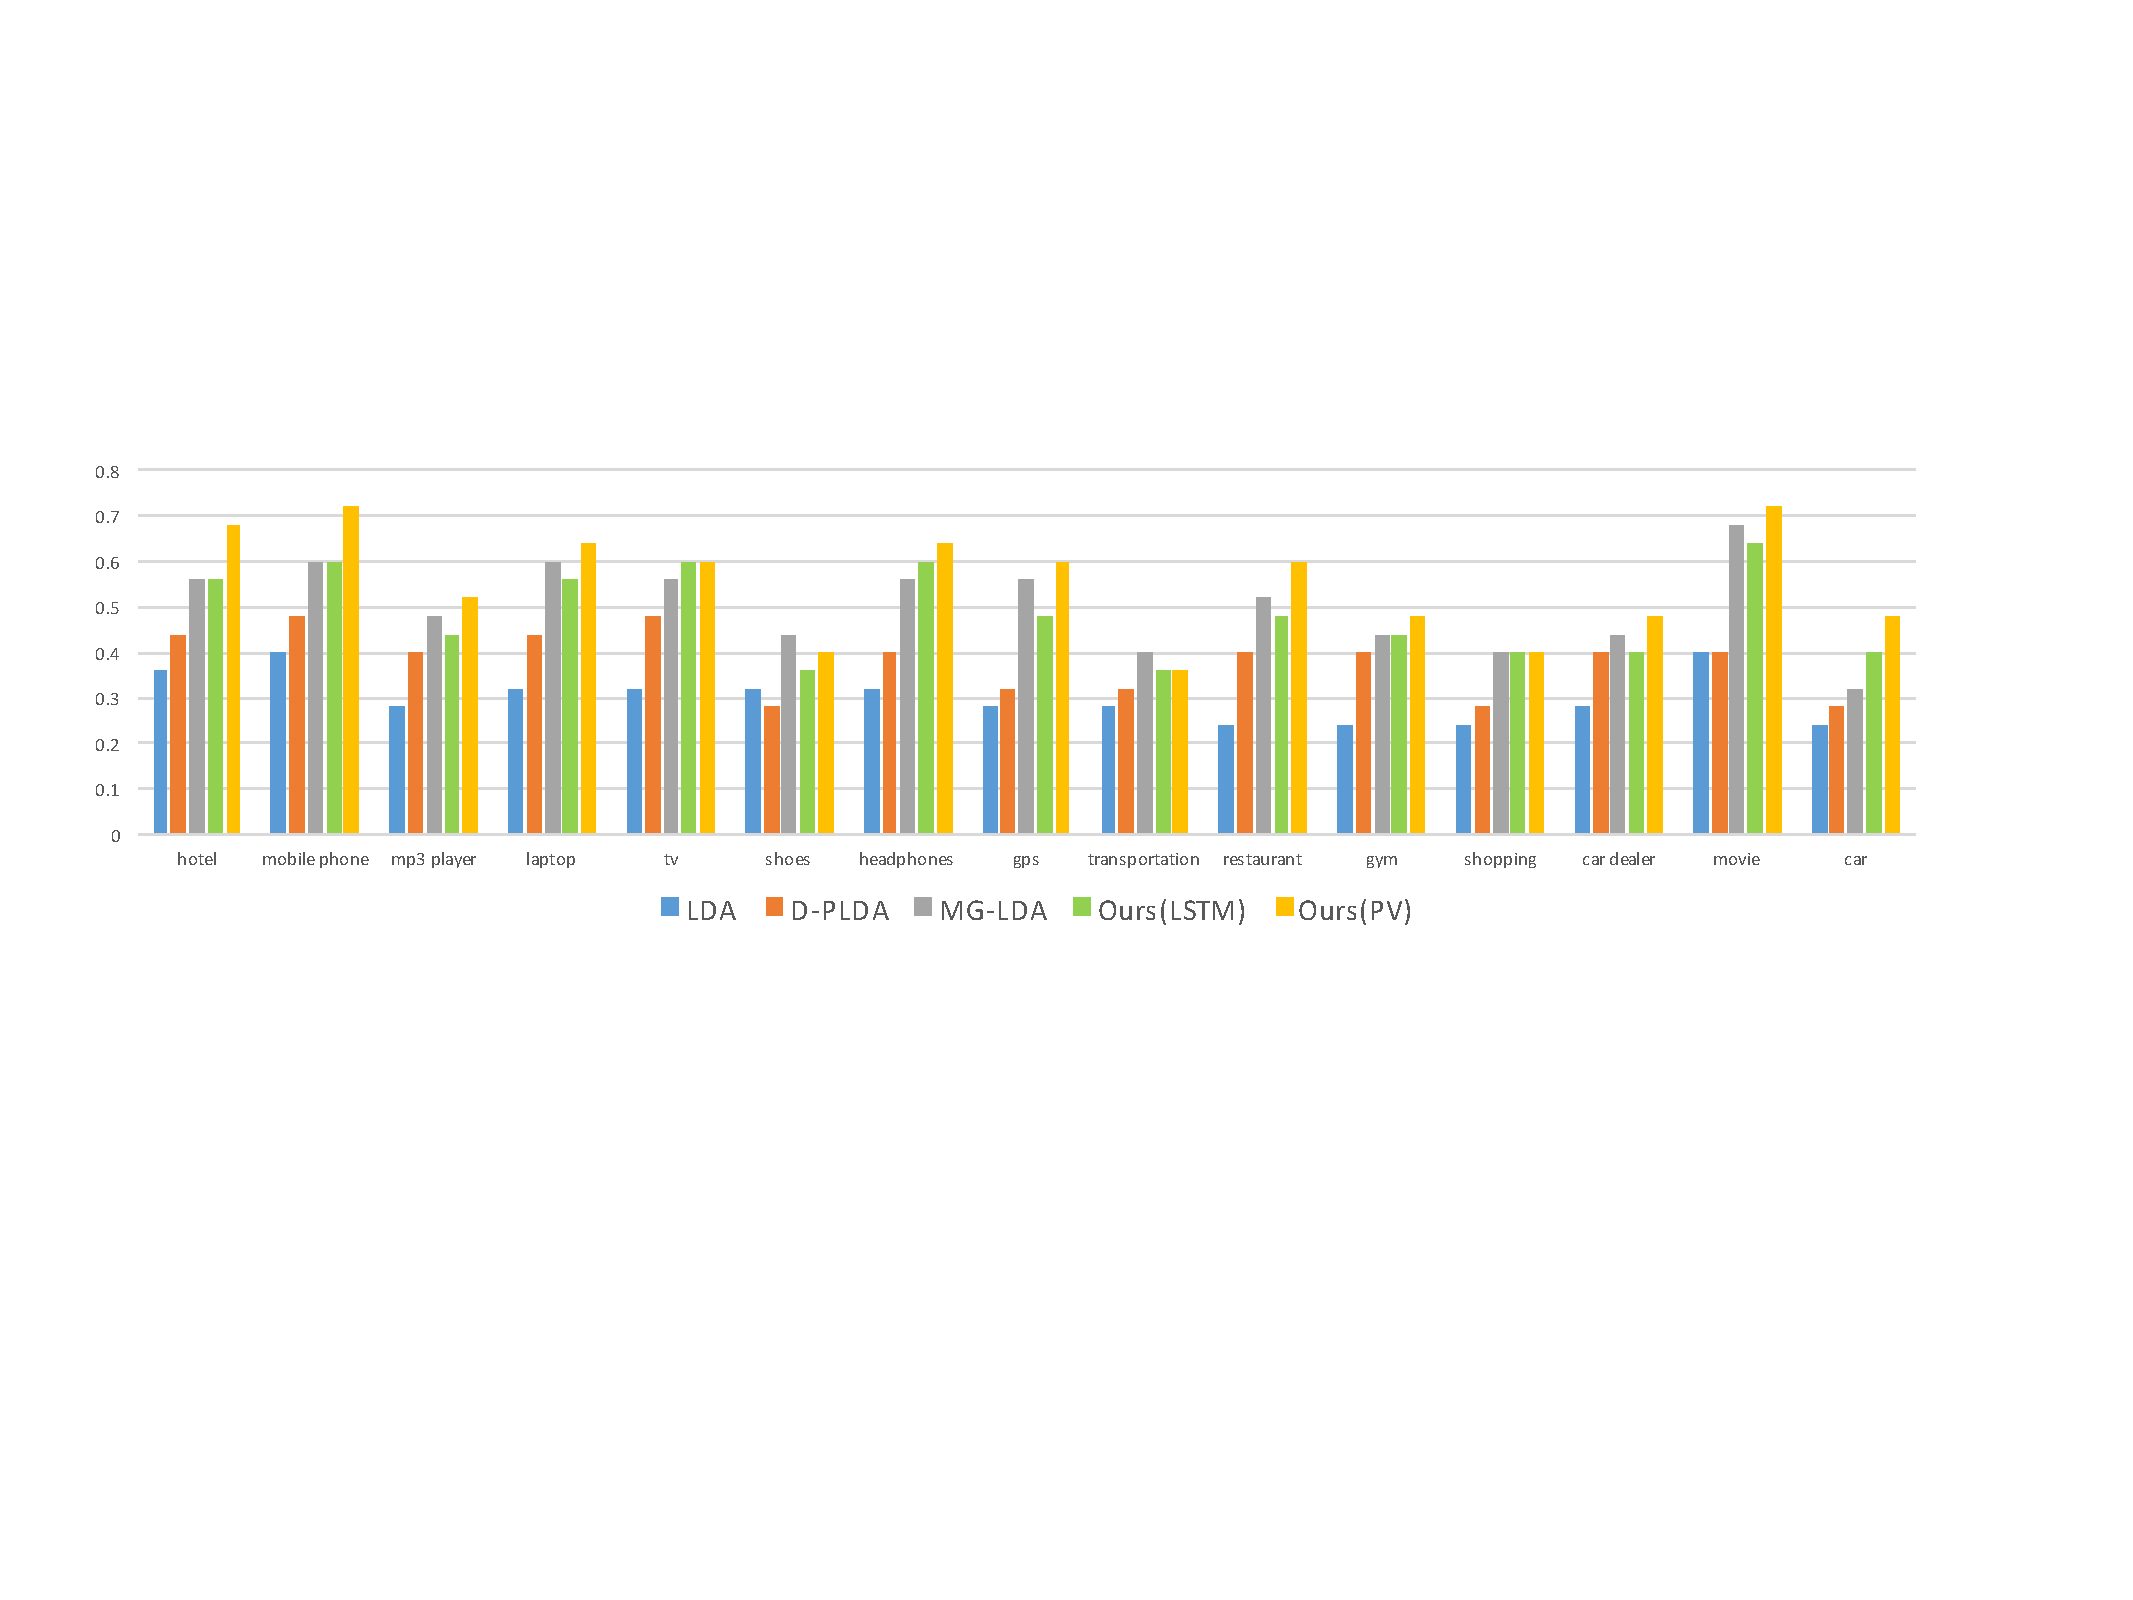
\includegraphics[width=2.0\columnwidth]{figures/results}
\caption{Comparison of accuracies from different models on aspect extraction.}
\label{fig:results}
\end{figure*}

In the end-to-end evaluation, we compare the performance of our models on aspect extraction with three other models as mentioned above. The results are shown in \figref{fig:results}. It can be seen that our model out-performed all other models in most of the categories (13 out of 15 with 2 ties). 
Our model with paragraph vector performs better than with LSTM, 
which is consistent to our result from the previous experiment.

We show the aspect word clusters on hotel reviews in \tabref{table:hotel_aspect_words}. The top words, which are chosen as the representatives of the aspects, are shown in boldface. 

\begin{table}[th]
\centering
\caption{Top aspect words for hotel reviews by different models}
\label{table:hotel_aspect_words}
\begin{tabular}{|l|l|} \hline
\multirow{5}{*}{Ours(PV)}
& \textbf{staff}, service, room, front, desk, check, concierge \\
& \textbf{food}, breakfast, bar, restaurant, coffee, morning, tea \\
& \textbf{price}, room, night, place, rate, service, money, star \\
& \textbf{room}, bed, bathroom, size, suite, floor, view, bedroom \\
& \textbf{location}, minute, square, subway, street, block, distance \\\hline

\multirow{5}{*}{Ours(LSTM)}
& \textbf{service}, front, desk, reception, concierge, check, gust \\
& \textbf{location}, station, minute, tube, station, bus, distance \\
& \textbf{time}, check, day, desk, charge, book, front, hour, night \\
& \textbf{food}, coffe, buffet, morning, tea, room, fruit, egg, juice \\
& \textbf{bed}, bathroom, size, floor, view, suite, king, book, decor \\ \hline

\multirow{5}{*}{MG-LDA}
& \textbf{shower}, bathroom, room, floor, area, bedroom, desk, tea \\
& \textbf{time}, day, room, check, front, desk, night, service \\
& \textbf{food}, bar, service, breakfast, restaurant, staff, taxi \\
& \textbf{room}, bed, floor, place, air, night, bathroom, noise \\
& \textbf{price}, business, service, star, internet, location, staff \\\hline

\multirow{5}{*}{DP-LDA}
& \textbf{service}, front, desk, reception, concierge, check, guest \\
& \textbf{station}, minute, tube, location, bus, distance, street \\
& \textbf{check}, day, time, desk, charge, book, front, hour \\
& \textbf{coffee}, buffet, morning, tea, room, day, fruit, food \\
& \textbf{bed}, bathroom, size, floor, view, suite, king, book \\\hline

\multirow{5}{*}{LDA}
& \textbf{stay}, night, place, trip, time, weekend, night, hour \\
& \textbf{location}, square, street, place, restaurant, market, block \\
& \textbf{room}, bed, bathroom, size, tv, king, suite, pillow \\
& \textbf{staff}, service, desk, location, concierge, room, night \\
& \textbf{room}, floor, noise, view, night, water, door, bathroom \\\hline
\end{tabular}
\end{table}


\subsubsection{Effect of Number of Expected Aspects ($K$)}

To evaluate the effect of different numbers of expected aspects, $K$, 
we ask our annotators to provide different numbers of labels on two categories. 
The number of aspects range from three to seven. 
The performance of the four models when changing the number of aspects are 
shown in \figref{fig:differentk}. 
It can be seen that our model performs constantly better than all other 
models regardless of the number of expected aspects. 

\begin{figure}[t!]
\centering
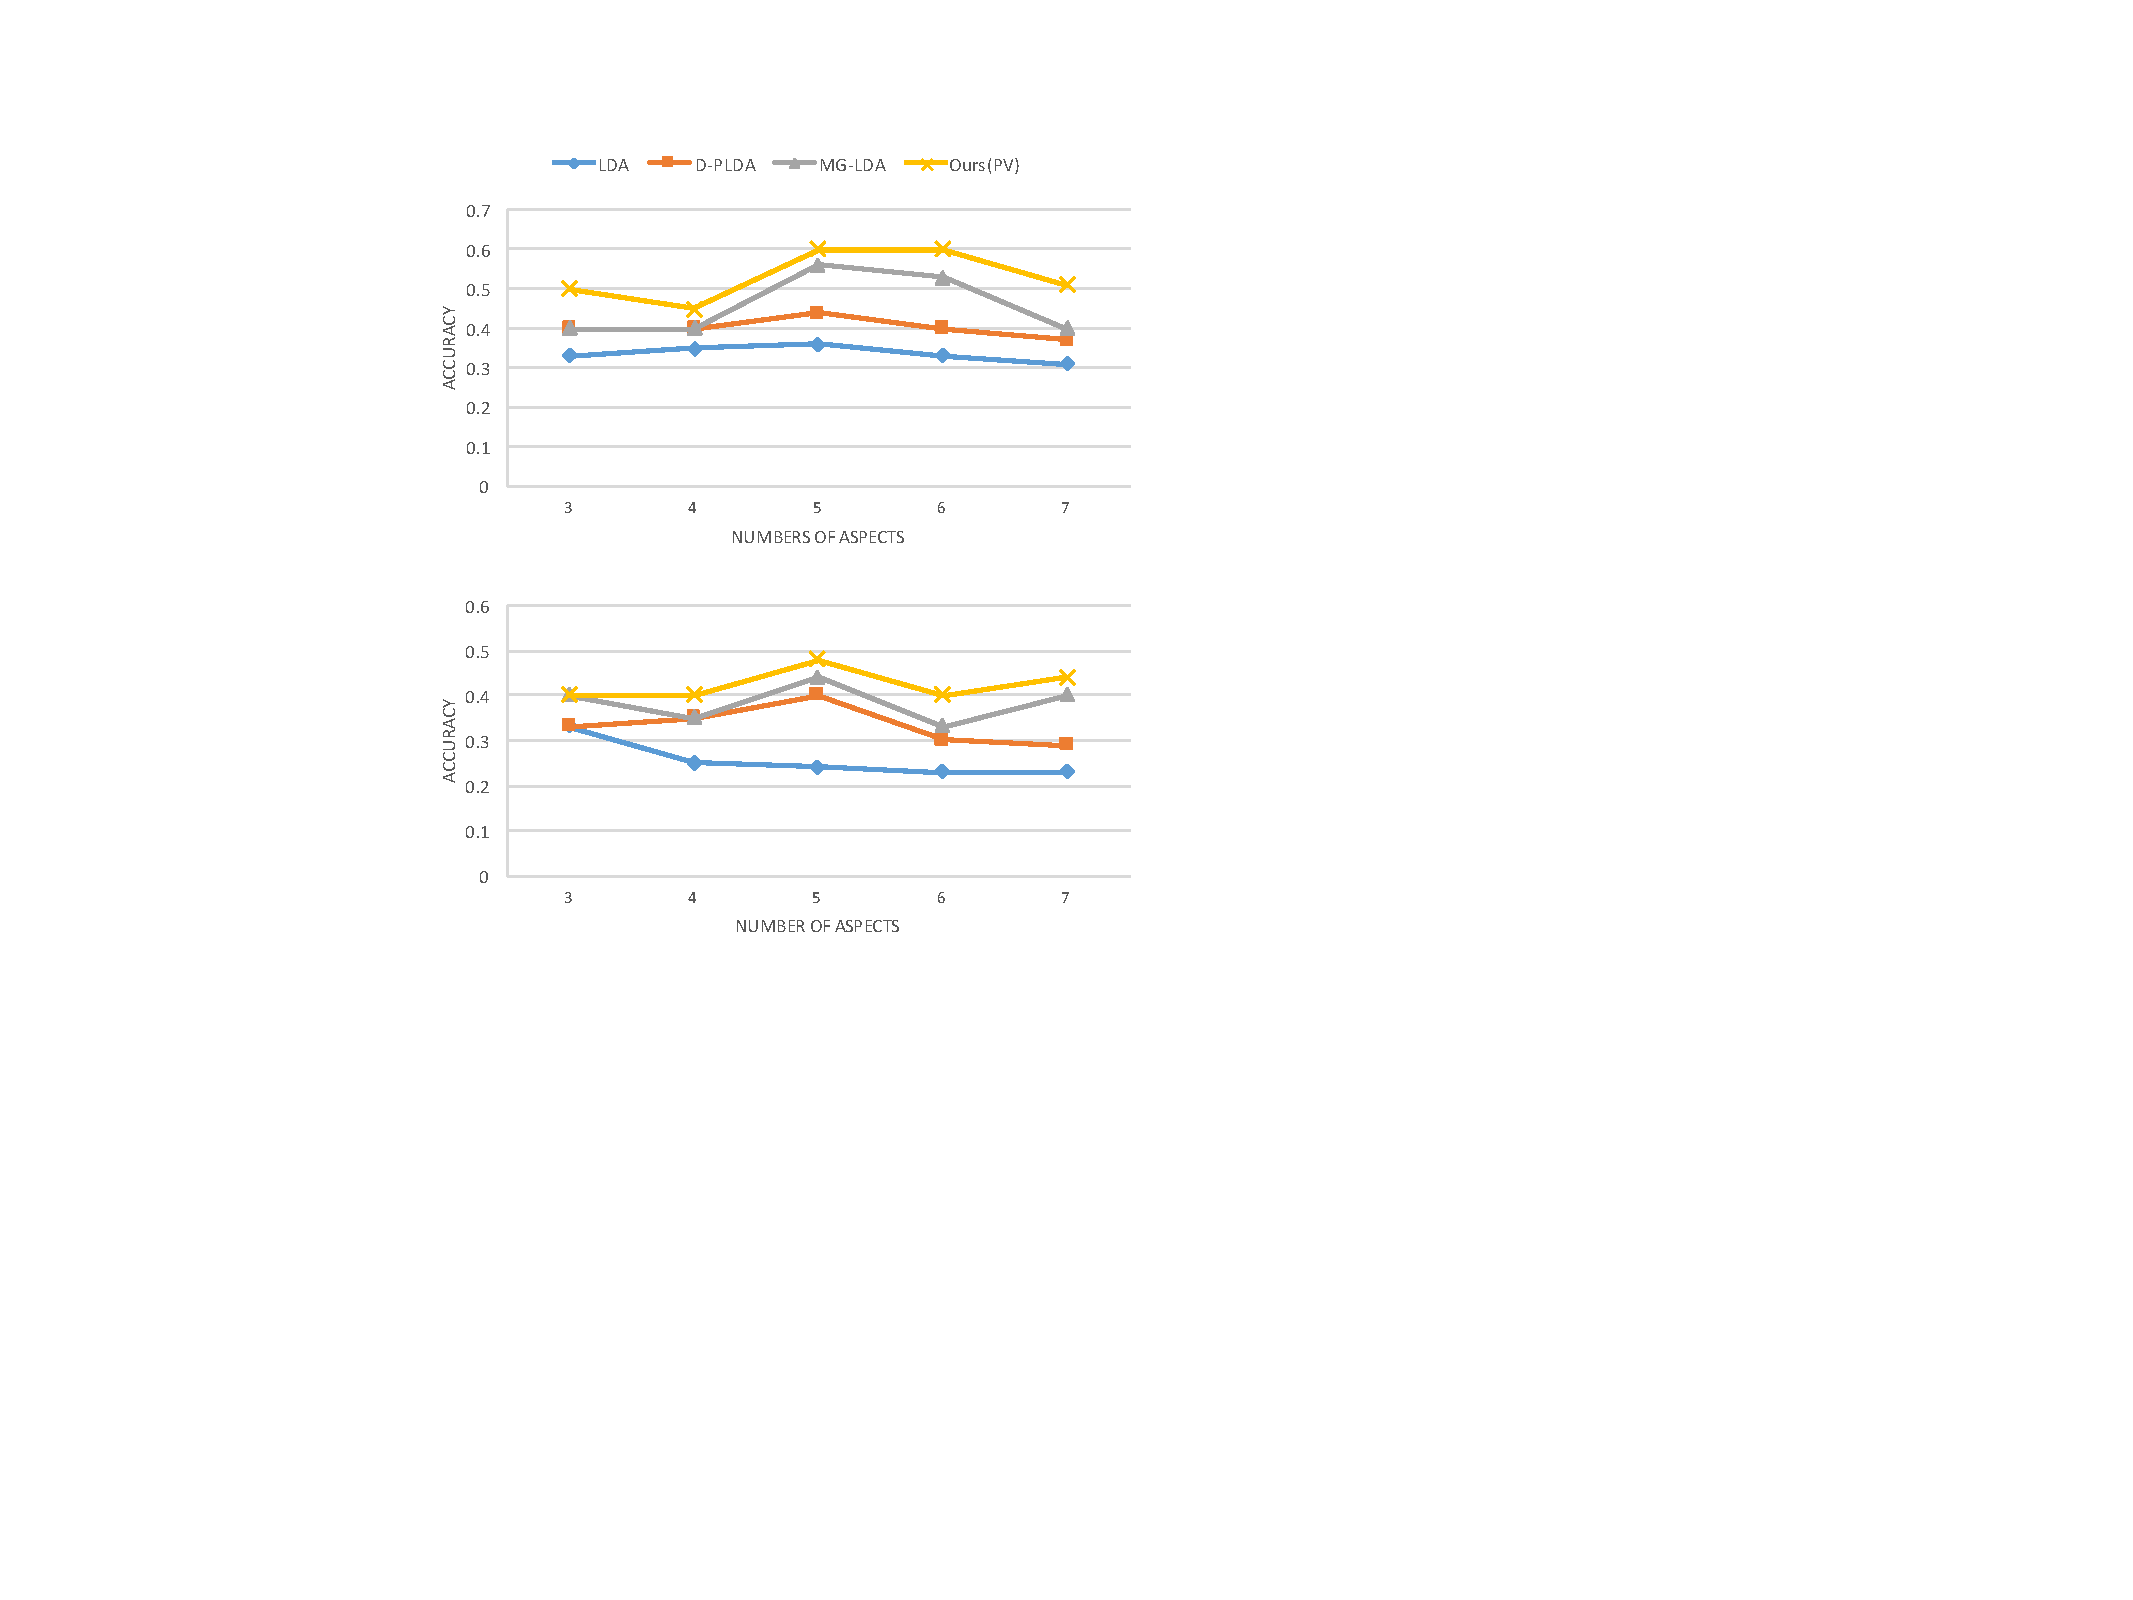
\includegraphics[width=0.9\columnwidth]{figures/differentk}
\caption{The performance of different models when varying the number of 
expected aspects. Top: hotel reviews. Bottom: gym reviews.}
\label{fig:differentk}
\end{figure}



\subsubsection{Effectiveness of Ranking}

Here we test the effectiveness of several techiques proposed for 
the ranking steps.
We compare three setups:
\begin{itemize}
    \item No word ranking. 
          Use directly the aspect cluster after step 3, aspect inference. 
          Remove redundant clusters with cluster ranking.
    \item No duplicate prevention.
          As mentioned in \secref{sec:word_ranking}, we do duplicate prevention
          by considering other clusters when ranking words within a cluster.
          In this setup we do not include this effort.
    \item Use all ranking methods.
\end{itemize}

The results are shown in \figref{fig:rankingeffect}.
The ranking scheme we propose, that is, work ranking with duplicate prevention,
has clear advantage over the other two across all product categories.

\begin{figure*}[th]
\centering
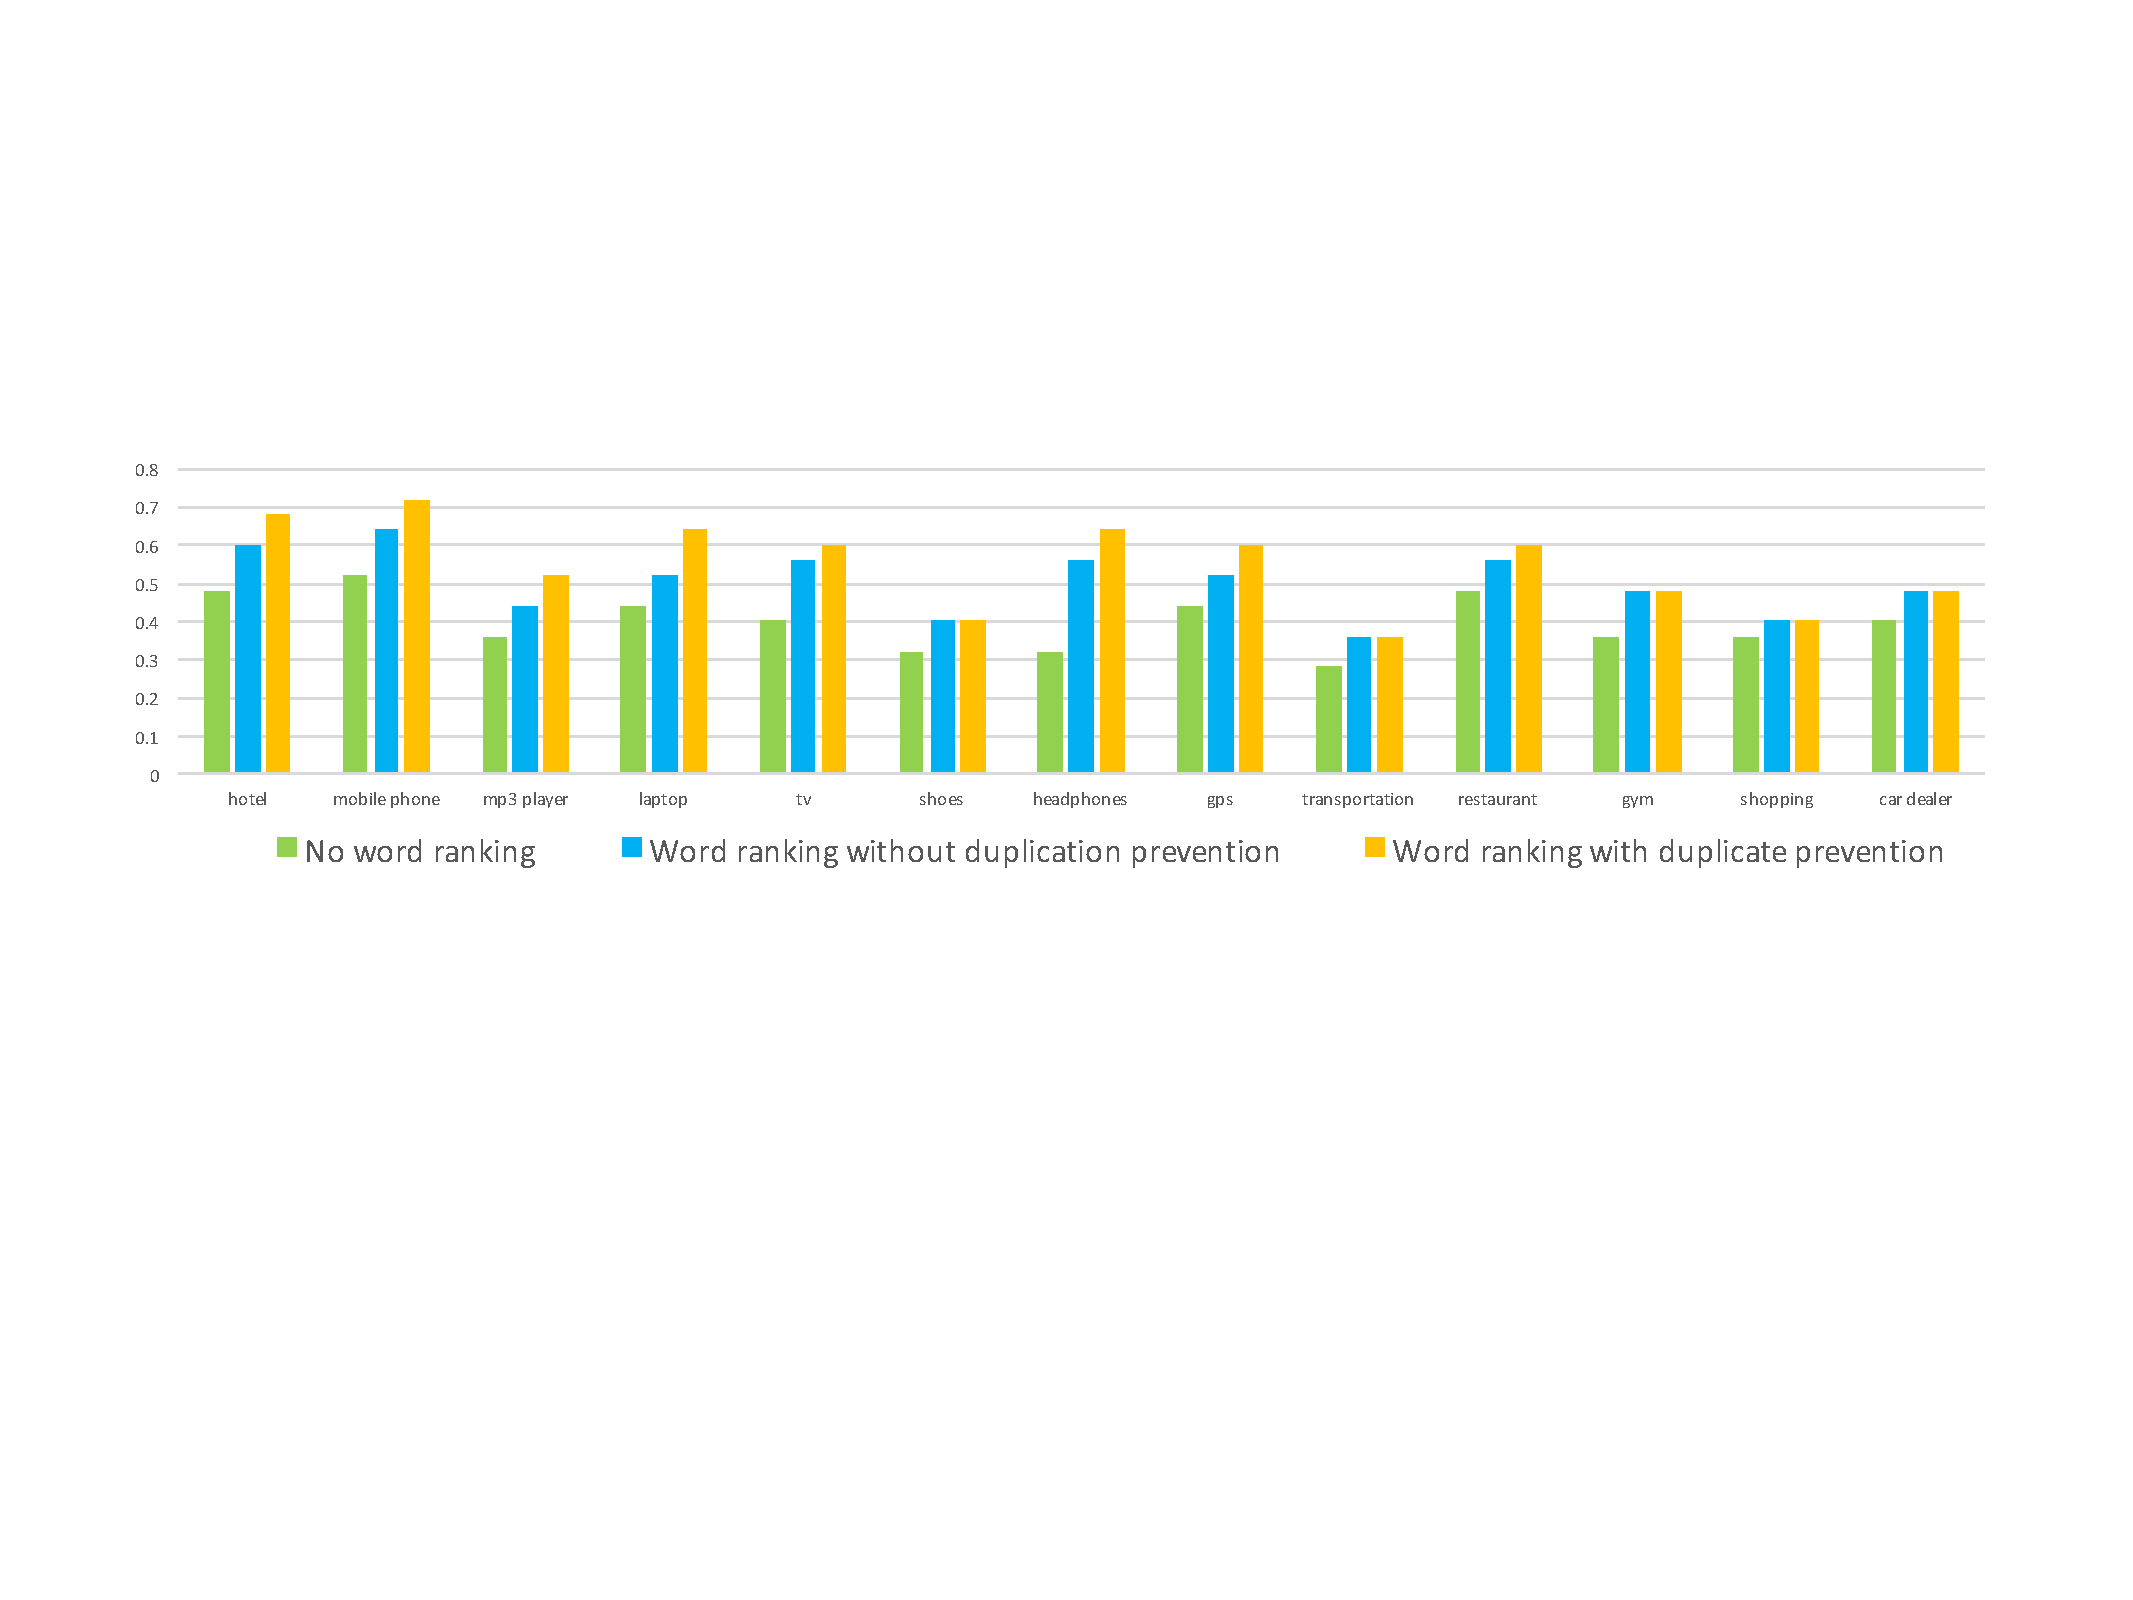
\includegraphics[width=2.0\columnwidth]{figures/rankingeffect}
\caption{The accuracy performance with different ranking setups.}
\label{fig:rankingeffect}
\end{figure*}



\subsection{Experiment 4: Aspect-based Review Summarization}
\label{sec:exp4}

In the last experiment,
we demonstrate how to use our proposed aspect 
extraction model to construct a complete aspect-based review summarization. 
We use the top aspect words extracted by our model as the basis 
for summarization, then predict the sentiment scores using a recurrent 
neural network. Note that this summarization can be produced by 
either a set of reviews or a single reivew. In this experiment, 
we use our method to extract the aspects for mobile phones, 
and produce aspect-based review summarization for 
two different models of mobile phone, namely Samsung Galaxy Core Prime 
and Apple iPhone 6.

\begin{table}[th]
\centering
\caption{The aspect clusters generated from mobile phone reviews}
\label{table:clusters}
\begin{tabular}{|l|}
\hline
\textbf{screen}, resolution, touch, display, color, picture \\ \hline
\textbf{battery}, power, charge, day, cable, charger \\ \hline
\textbf{quality}, break, day, build, buy, control \\ \hline
\textbf{service}, buy, check, help, website, shipping \\ \hline
\textbf{price}, money, worth, cost, charge, free \\ \hline
\textbf{design}, color, metal, case, plastic, silver \\ \hline
\end{tabular}
\end{table}

The aspect clusters by our method on the mobile phone review data 
is shown in \tabref{table:clusters}. Since the aspects are shared across 
all the products within the same category, 
we apply our model on the whole mobile 
phone review dataset to extract these aspects. 
Then we focus on the reviews for two specific models of mobile phone 
and process them with a sentiment prediction backend.

We use the aspect clusters shown in the above table to identify the 
aspects in the review sentences by checking if the top aspect words 
in each cluster appeared. If so, the sentence is attached with weight 
equal to the highest aspect score it contains. Further, the sentiment 
value of the sentence is predicted with an LSTM and feed-woward network 
model trained on Stanford Sentiment Treebank \cite{socher2013recursive}. 
The sentiment value for each aspect from the whole set is the 
weighted average of the predicted sentiment values.

The final aspect-based review summarization of two different mobile phones 
are shown in \figref{fig:experiments:comparison}. 
With this summarization, users can easily compare different products 
with respect to the same set of important aspects, without having to 
read a lot of reviews.

\begin{figure}[th]
\centering
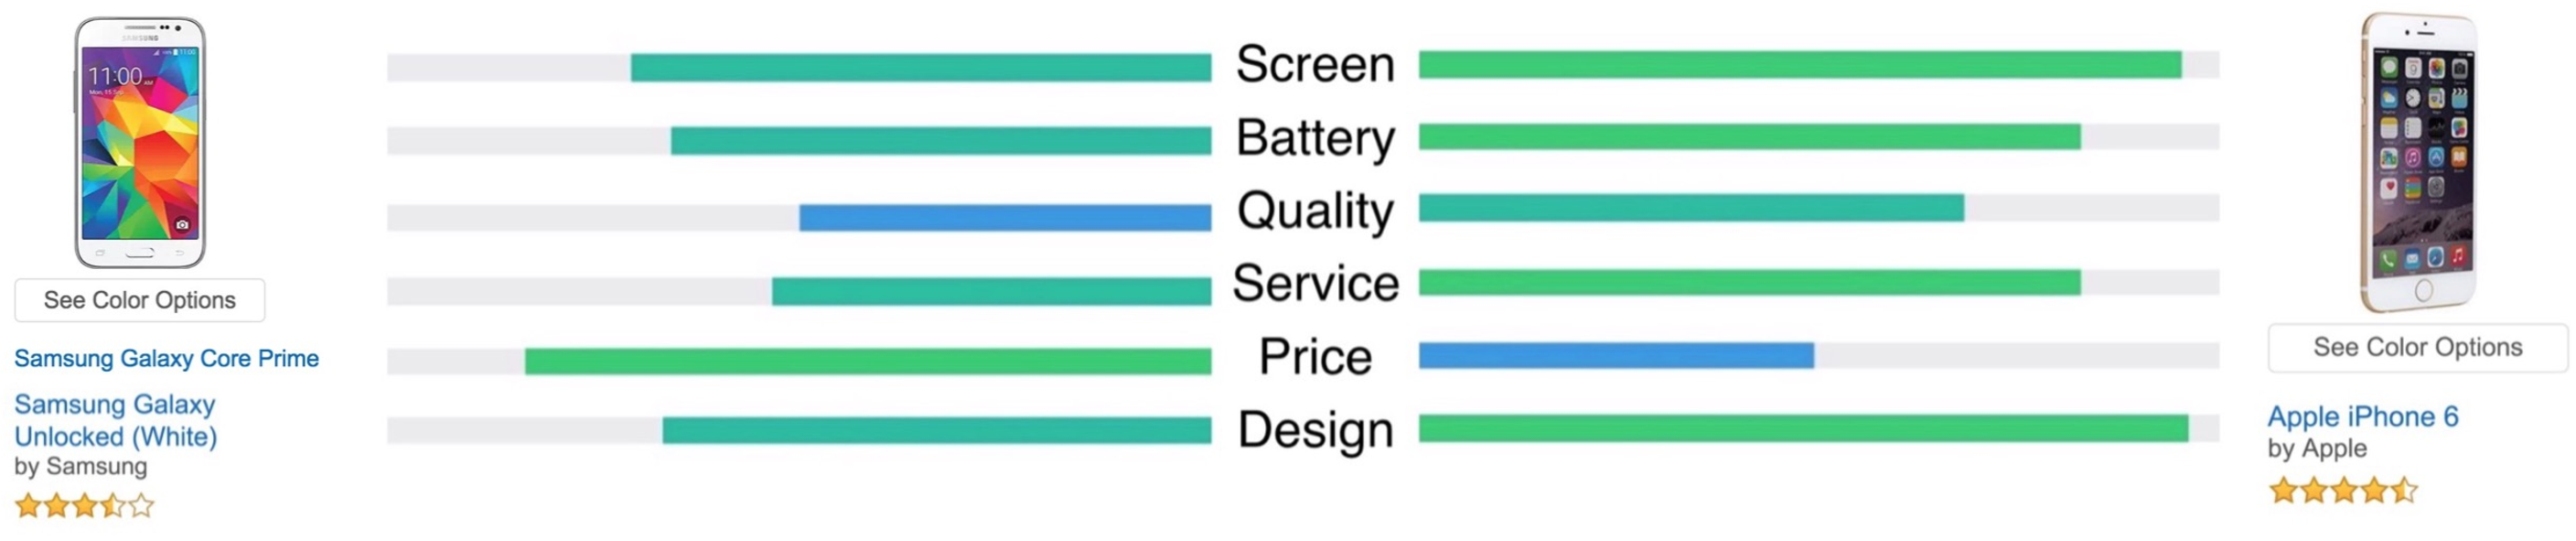
\includegraphics[width=1.0\columnwidth]{figures/comparison}
\caption{Comparing two mobile phones.}
\label{fig:experiments:comparison}
\end{figure}

%\KZ{Where should the following para go? Doesn't seem very relevant to
%experiment 3. Is it a summary of the whole section? Then shouldnt start
%with Another...}
One of the advantages of using our method for review summarization
is that the chosen aspects 
reflect what the consumers care most about each product type. 
The fundamental reason behind this is that our model can truly leverage 
the large amount of data compared to traditional methods. 
In \figref{fig:phrases}, we can see phrases such as ``beautiful screen'' 
and ``good camera'', but we also see ``high resolution'', which 
is confusing because we cannot know if it means the screen or the camera, 
and either way there is overlap in meaning. In our method, the topics of 
the sentence is implicitly embedded in the sentence vector in the first 
clustering process, so we can leverage not only the opinion phrases 
but other surrounding words to decide whether ``high resolution'' 
refers to the screen or the camera. For example, if the review 
sentence is ``it has high resolution and the texts look so crisp'', 
we would know it's about the screen. This allows our summarization to 
leverage a lot more data than these traditional methods. 
